\documentclass{beamer}

%
% Choose how your presentation looks.
%
% For more themes, color themes and font themes, see:
% http://deic.uab.es/~iblanes/beamer_gallery/index_by_theme.html
%
\mode<presentation>
{
  \usetheme{default}      % or try Darmstadt, Madrid, Warsaw, ...
  \usecolortheme{default} % or try albatross, beaver, crane, ...
  \usefonttheme{default}  % or try serif, structurebold, ...
  \setbeamertemplate{navigation symbols}{}
  \setbeamertemplate{caption}[numbered]
  \setbeamertemplate{footline}[page number]
  \setbeamercolor{frametitle}{fg=white}
  \setbeamercolor{footline}{fg=black}
} 

\usepackage[english]{babel}
\usepackage[utf8x]{inputenc}
\usepackage{tikz}
\usepackage{listings}
\usepackage{courier}
\usepackage{minted}

\xdefinecolor{darkblue}{rgb}{0.1,0.1,0.7}
\xdefinecolor{dianablue}{rgb}{0.18,0.24,0.31}
\definecolor{commentgreen}{rgb}{0,0.6,0}
\definecolor{stringmauve}{rgb}{0.58,0,0.82}

\lstset{ %
  backgroundcolor=\color{white},      % choose the background color
  basicstyle=\ttfamily\small,         % size of fonts used for the code
  breaklines=true,                    % automatic line breaking only at whitespace
  captionpos=b,                       % sets the caption-position to bottom
  commentstyle=\color{commentgreen},  % comment style
  escapeinside={\%*}{*)},             % if you want to add LaTeX within your code
  keywordstyle=\color{blue},          % keyword style
  stringstyle=\color{stringmauve},    % string literal style
  showstringspaces=false,
  showlines=true
}

\lstdefinelanguage{scala}{
  morekeywords={abstract,case,catch,class,def,%
    do,else,extends,false,final,finally,%
    for,if,implicit,import,match,mixin,%
    new,null,object,override,package,%
    private,protected,requires,return,sealed,%
    super,this,throw,trait,true,try,%
    type,val,var,while,with,yield},
  otherkeywords={=>,<-,<\%,<:,>:,\#,@},
  sensitive=true,
  morecomment=[l]{//},
  morecomment=[n]{/*}{*/},
  morestring=[b]",
  morestring=[b]',
  morestring=[b]"""
}

\title[2016-09-30-gpudb]{GPU-enabled physics event database}
\author{Jim Pivarski}
\institute{Princeton -- DIANA}
\date{September 30, 2016}

\begin{document}

\logo{\pgfputat{\pgfxy(0.11, 8)}{\pgfbox[right,base]{\tikz{\filldraw[fill=dianablue, draw=none] (0 cm, 0 cm) rectangle (50 cm, 1 cm);}}}\pgfputat{\pgfxy(0.11, -0.6)}{\pgfbox[right,base]{\tikz{\filldraw[fill=dianablue, draw=none] (0 cm, 0 cm) rectangle (50 cm, 1 cm);}
\includegraphics[height=0.99 cm]{diana-hep-logo.png}\tikz{\filldraw[fill=dianablue, draw=none] (0 cm, 0 cm) rectangle (4.9 cm, 1 cm);}}}}

\begin{frame}
  \titlepage
\end{frame}

\logo{\pgfputat{\pgfxy(0.11, 8)}{\pgfbox[right,base]{\tikz{\filldraw[fill=dianablue, draw=none] (0 cm, 0 cm) rectangle (50 cm, 1 cm);}
\includegraphics[height=1 cm]{diana-hep-logo.png}}}}

% Uncomment these lines for an automatically generated outline.
%\begin{frame}{Outline}
%  \tableofcontents
%\end{frame}

\begin{frame}{Current physics workflow}
\vspace{0.5 cm}
\only<1>{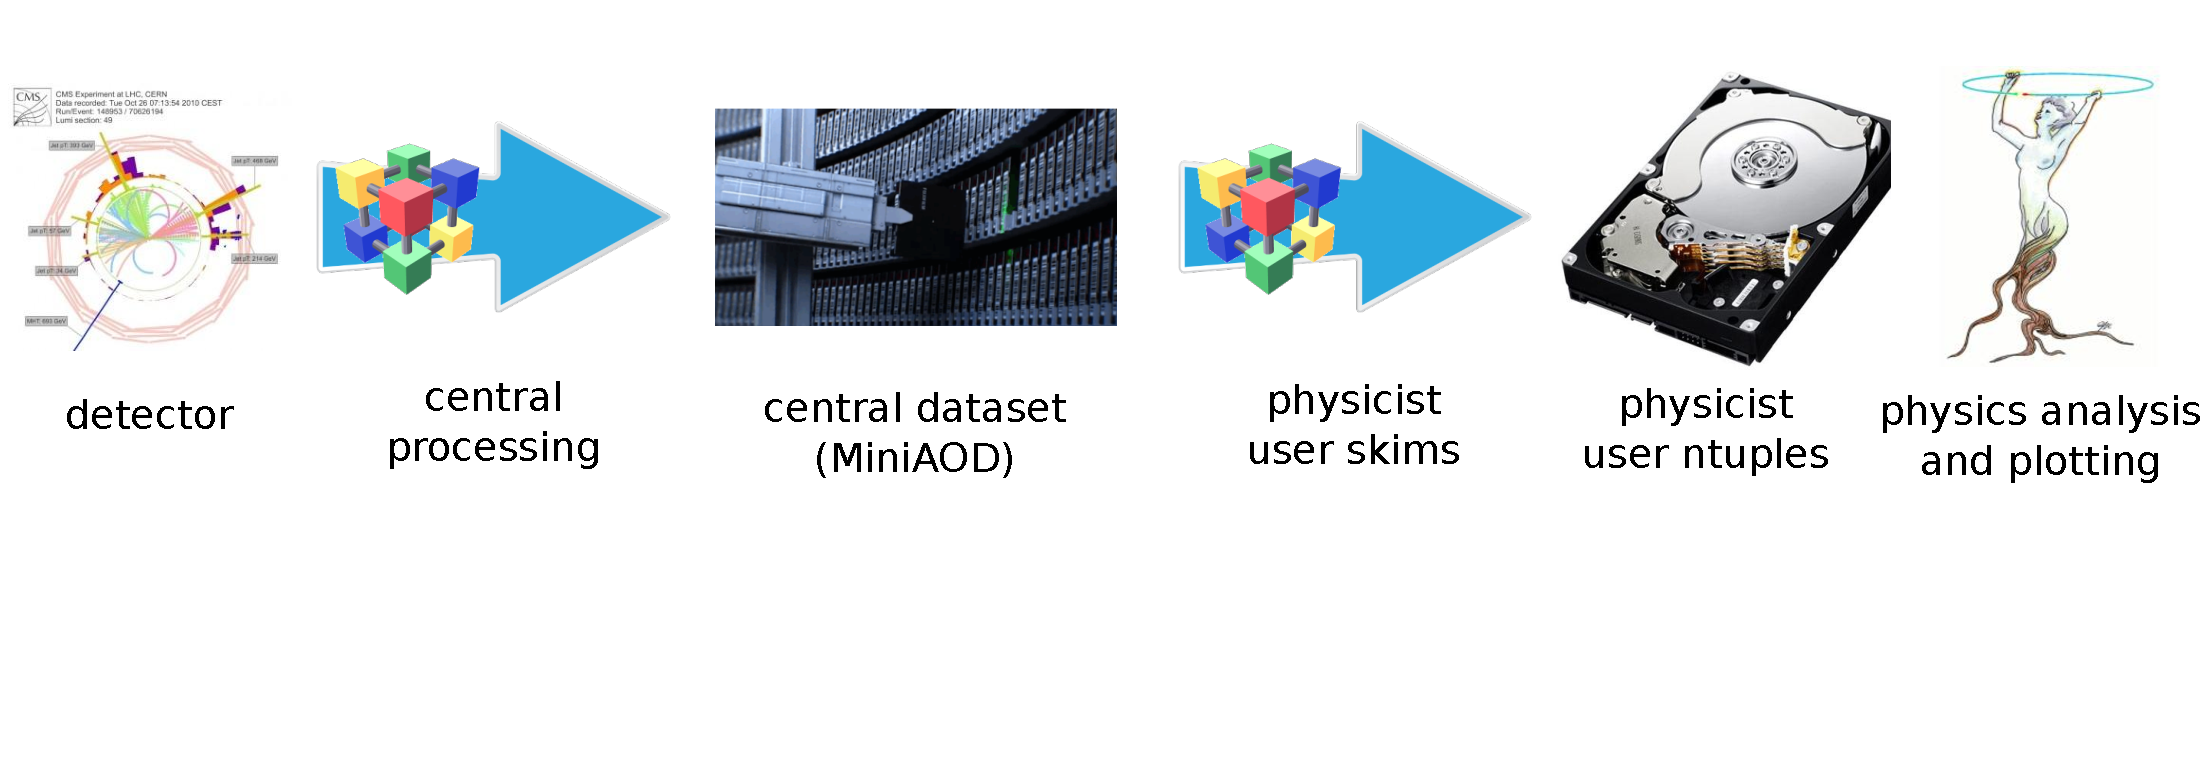
\includegraphics[width=\linewidth]{workflow1.pdf}}
\only<2->{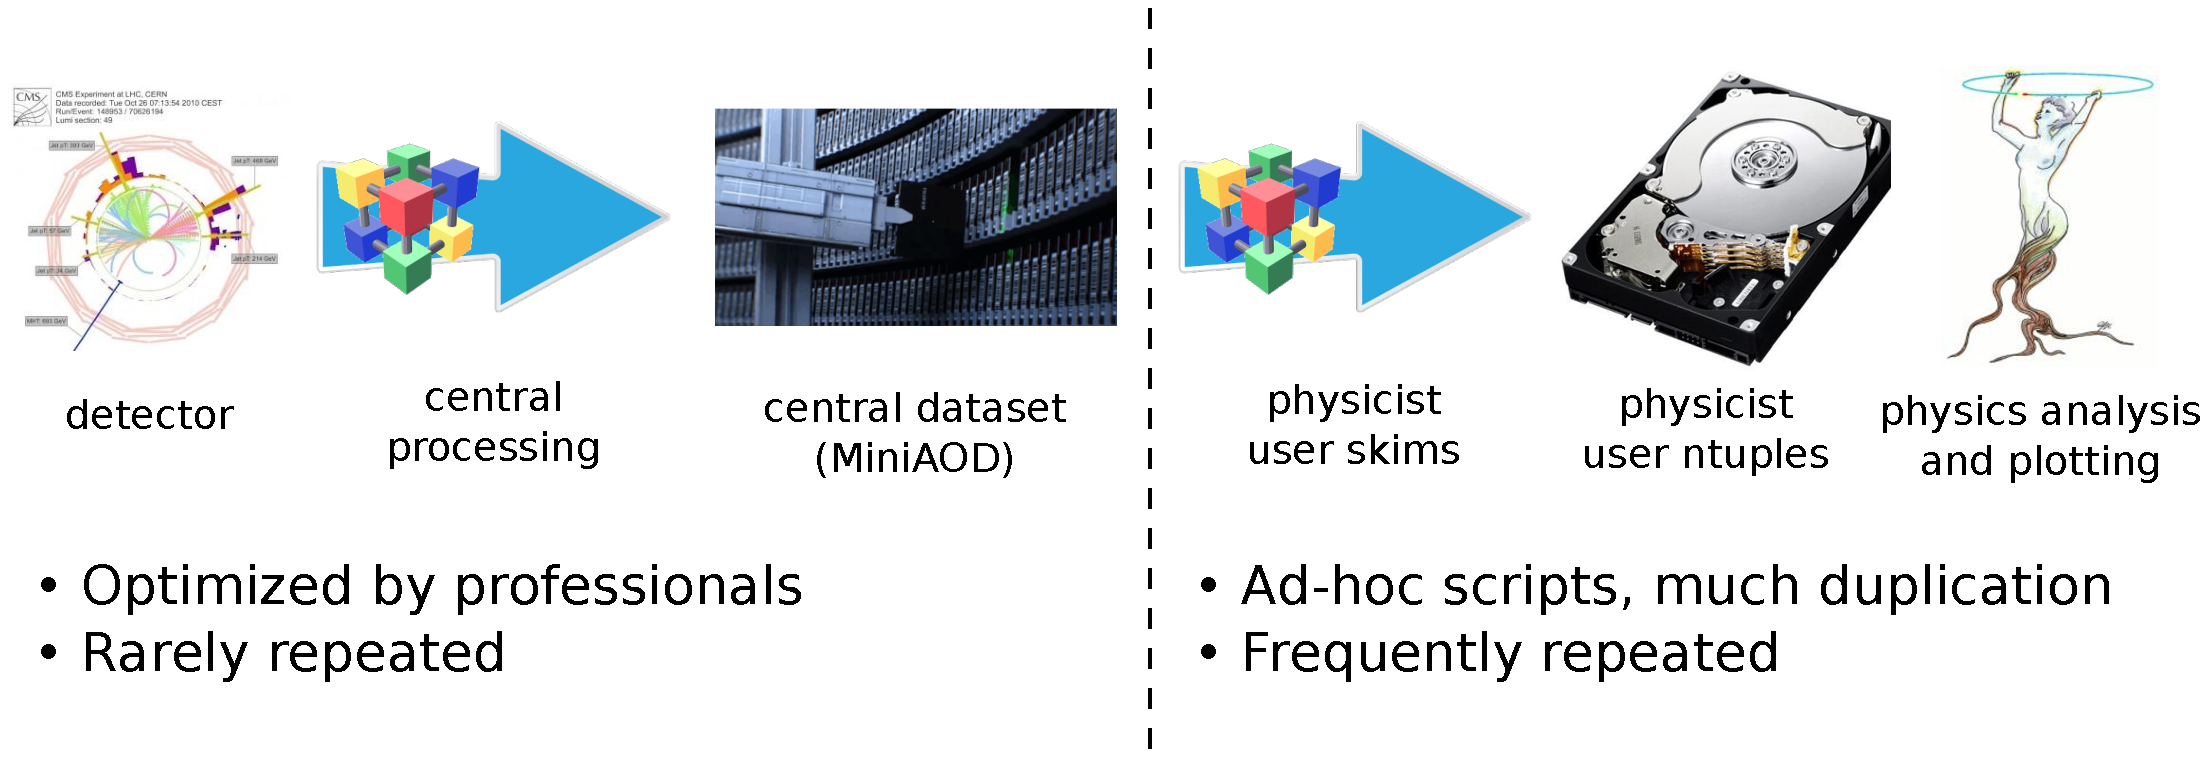
\includegraphics[width=\linewidth]{workflow2.pdf}}

\vspace{0.25 cm}
\begin{itemize}
\item<3-> Event index database addresses one part of the slowness of physicist user skims at a cost of adding a layer of complexity.
\item<4-> I am now discovering that there are much worse hotspots in the physicists' scripts.
\item<5-> Bugs and inefficiencies in the custom code and ntuple-version control issues get in the way of physicists doing analysis.
\end{itemize}
\end{frame}

\begin{frame}{Ideal physics workflow}
\vspace{0.5 cm}
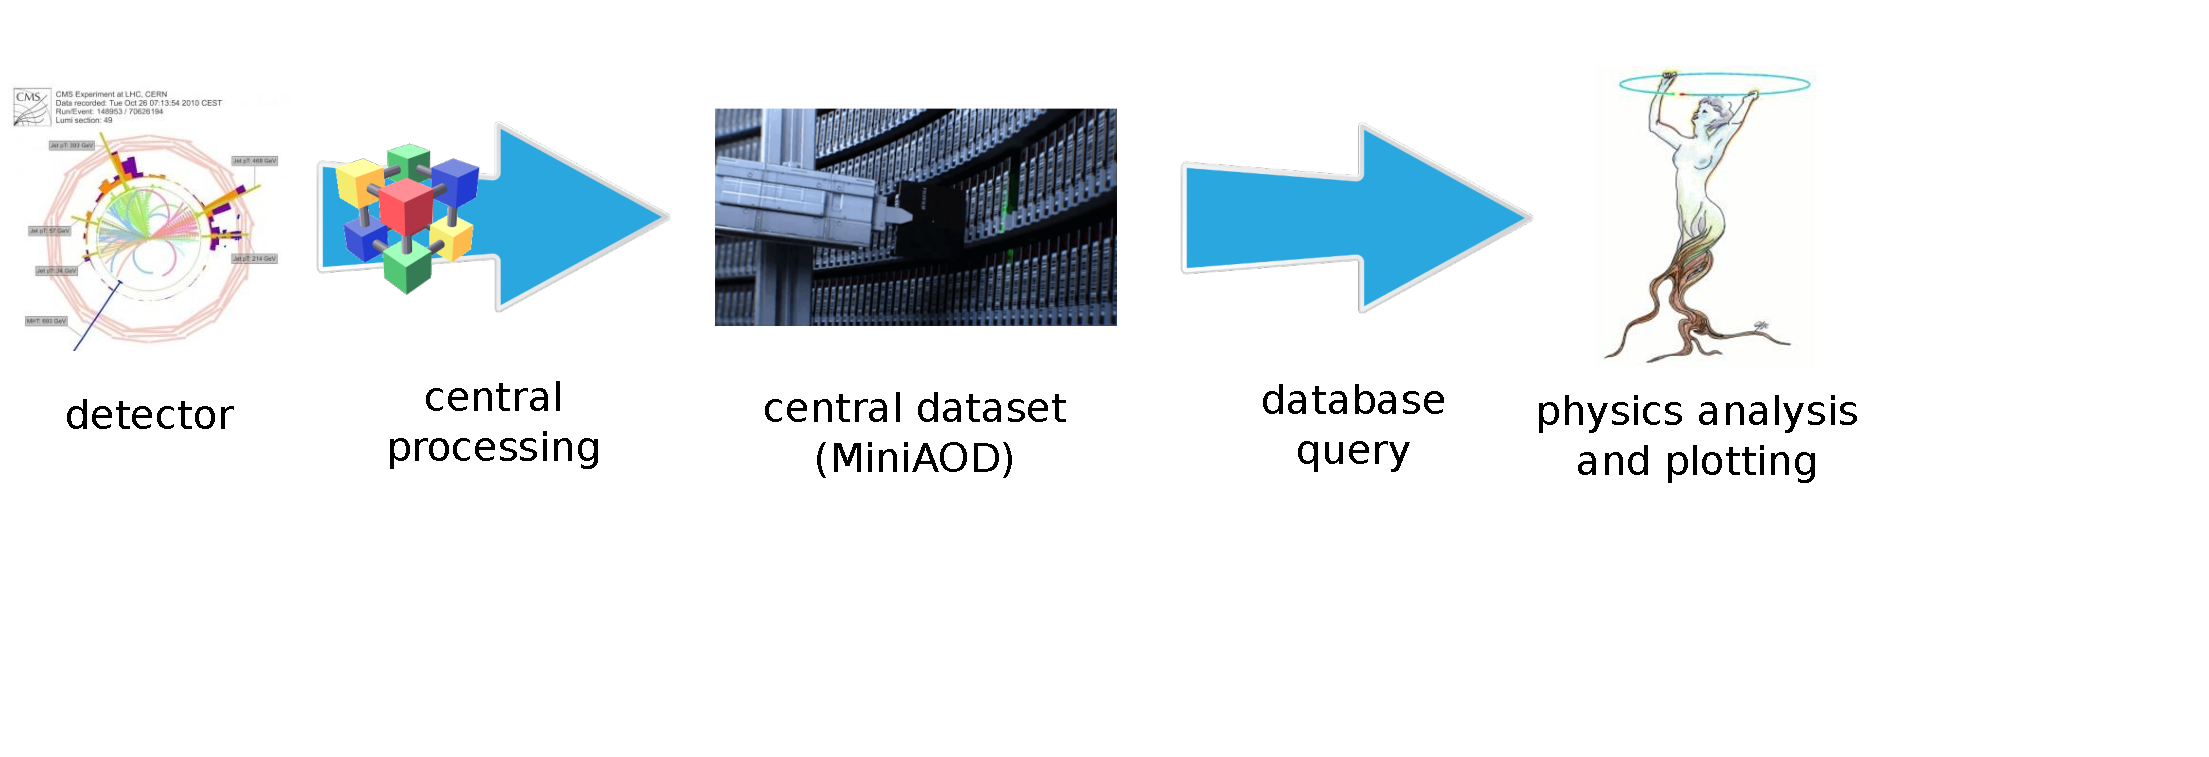
\includegraphics[width=\linewidth]{workflow3.pdf}

\vspace{0.25 cm}
\begin{itemize}
\item Ideally, data should go directly from centralized dataset into plots and statistical routines.
\item<2-> But as we've seen, physics data are too deeply structured for traditional database indexing.
\end{itemize}

\vspace{1 cm}
\end{frame}

\begin{frame}{Ways to get the data}
\vspace{0.25 cm}
\small
\begin{description}\setlength{\itemsep}{0.2 cm}
\item[Parallel scripts (current):] run many tasks on the GRID, each pulls data over the network, analyzes every event; filters, computes quantities of interest.

\item[Relational database:]<2-> use pre-computed indexes over event data to avoid looking at every event in every query.

\vspace{0.1 cm}
But\ldots\ how to index over nested structures? Normal form requires expensive joins.

\vspace{0.1 cm}
Something like this was tried in the 90's with Objectivity (BaBar, CLEO, maybe others): considered a failure.

\item[NoSQL databases:]<3-> many different types, but most would require even more expensive map-reduce jobs instead of joins.

\item[GPU database:]<4-> use massive parallelism on cached quantities.

\vspace{0.1 cm}
Similar to current approach in that every event is examined (no indexing), but data-fetch is shared among users.
\end{description}
\end{frame}

\begin{frame}{GRID jobs vs.\ GPU queries}
\vspace{0.25 cm}
\small
\begin{columns}[t]
\column{0.5\linewidth}
\textcolor{darkblue}{\underline{GRID jobs}}
\begin{enumerate}
\item Physicist Phil's job asks for a block of $p_x$ and $p_y$ from events 1000--1999.

XRootD supplies them.

\item Phil's C++ code selects half the events and computes $\sqrt{{p_x}^2 + {p_y}^2}$ for each. They are all saved to disk.

\item At the end of the job, the output file of $\mathcal{O}(N_{\mbox{\scriptsize events}})$ rows is sent back to Phil.

\item Physicist Phoebe's job asks for a block of $p_x$, $p_y$, and $p_z$ from events 1000--1999.

\textcolor{darkblue}{XRootD supplies them \mbox{all again.\hspace{-1 cm}}}
\end{enumerate}

\column{0.5\linewidth}
\textcolor{darkblue}{\underline{GPU queries}}
\begin{enumerate}
\item Physicist Phil's query requires a block of $p_x$ and $p_y$.

They are loaded into the GPU's global memory.

\item Phil's filter and transformation have been converted into GPU kernels that operate on all events in the block at once.

\item At the end of the query, only aggregate quantities are returned: e.g.\ a histogram.

\item Physicist Phoebe's query requires $p_x$, $p_y$, and $p_z$.

\textcolor{darkblue}{Only loads $p_z$ into the GPU; \\ $p_x$ and $p_y$ are already there.}
\end{enumerate}
\end{columns}
\end{frame}

\begin{frame}{GRID jobs vs.\ GPU queries}
\vspace{0.5 cm}
\begin{block}{Main advantages of GPU}
\begin{itemize}
\item Tasks are more lightweight, less overhead in parallelization.
\item Commonly used quantities stay in GPU-cache between user's job and the next.

\vspace{0.1 cm}
Popular data are faster to query than less popular data.
\end{itemize}
\end{block}

\begin{block}{Disadvantages of GPU}
\begin{itemize}
\item Queries have to be compiled into kernels. A new language will be required (we don't want to execute unrestricted CUDA) and that language will have limited capabilities.
\item For cache to be useful, jobs must have good data locality.
\end{itemize}
\end{block}
\end{frame}

\begin{frame}{Feasibility}
\vspace{0.25 cm}
\begin{itemize}
\item Princeton's Tiger cluster is an example of what can be built. \textcolor{gray}{\small (But how much did it cost? I need to look that up.)}

\small
\hfill \begin{tabular}{p{0.9\linewidth}}
50 computers \\
4 GPUs per computer \\
5 GB global memory per GPU (total of 1 TB GPU cache) \\
824 GB of RAM per CPU (total of 41 TB)
\end{tabular}

\normalsize
\item<2-> CPU RAM to GPU global memory (for cache misses)
\begin{itemize}
\item cheap gaming cards: 1 GB/s \textcolor{gray}{$\to$ 30 seconds to fill {\it entire} GPU}
\item pinned memory is 50\% faster (my tests)
\item NVLink for supercomputers: 80 GB/s
\item loading data for obscure queries can be concurrent with running common queries.
\end{itemize}

\item<3-> Data to CPU RAM
\begin{itemize}
\item mechanical hard drives: 0.2 GB/s
\item SSDs: 0.2--1.5 GB/s
\item network: $\sim$1--10 GB/s, but remember that jobs must have good data locality.
\end{itemize}

\end{itemize}
\end{frame}

\begin{frame}{Data locality}
\begin{description}
\item[``HDFS style''] blocks of data are located on the task executors; tasks go to the executors that have the required data.
\item[``XRootD style''] data source and task executors are distinct, connected by fast network. Tasks go to any executor.
\end{description}

\begin{itemize}
\item<2-> Disadvantage of HDFS style: if some datasets are much more popular than others, tasks will not be load-balanced.
\item<3-> But failing to send tasks that require the same data to the same executor would render caching useless, so we {\it must} have HDFS style locality. \textcolor{gray}{(This system has ``Spark style'' caching.)}
\item<4-> Data distribution across cluster must be fine-grained.

\textcolor{gray}{(Don't put all the Higgs data on one machine!)}
\end{itemize}
\end{frame}

\begin{frame}[fragile]{Data representation}
\vspace{0.45 cm}
\small
\hspace{-0.35 cm}Logically, data events are trees with known schema:
\tiny
\begin{center}
\begin{minipage}{0.5\linewidth}
\begin{verbatim}
event
  |
  +--- primaryVertices: int
  +--- tracks: collection of records
  |      |
  |      +--- pt: float
  |      +--- theta: float
  |      +--- hits: collection of records
  |             |
  |             +--- charge: float
  |             +--- time: float
  |
  +--- showers: collection of records
         |
         +--- et: float
\end{verbatim}
\end{minipage}
\end{center}

\small
\hspace{-0.35 cm}Physically, each leaf should be an array of bytes. Ways to break it down:

\vspace{0.25 cm}
\tiny
\begin{columns}[t]
\column{0.5\linewidth}
{\bf Pointers to children}

\vspace{-0.35 cm}
\begin{verbatim}
primaryVertices      int     (one per event)
firstTrackId         long    (one per event)
numTracks            int     (one per event)
tracks.pt            float   (one per track)
tracks.theta         float   (one per track)
tracks.firstHitId    long    (one per track)
tracks.numHits       int     (one per track)
tracks.hits.charge   float   (one per hit)
tracks.hits.time     float   (one per hit)
firstShowerId        long    (one per event)
numShowers           int     (one per event)
showers.et           float   (one per shower)
\end{verbatim}

\column{0.5\linewidth}
{\bf Pointers to parents} (more data in fewer columns)

\vspace{-0.35 cm}
\begin{verbatim}
primaryVertices      int     (one per event)

tracks.eventId       long    (one per track)
tracks.pt            float   (one per track)
tracks.theta         float   (one per track)

tracks.hits.trackId  long    (one per hit)
tracks.hits.charge   float   (one per hit)
tracks.hits.time     float   (one per hit)

showers.eventId      long    (one per shower)
showers.et           float   (one per shower)
\end{verbatim}
\end{columns}
\end{frame}

\begin{frame}{Data representation\ldots\ considerations}
\vspace{0.5 cm}
\scriptsize
\begin{itemize}\setlength{\itemsep}{0.25 cm}
\item All columns associated with a given event must be loadable into the same GPU, but usually only a few columns would be loaded at any given time.

\item The event-level columns (e.g.\ {\tt primaryVertices}) have different lengths than the track-level columns (e.g.\ {\tt tracks.pt}). How to avoid memory fragmentation?

\item Should the data be pre-formatted, avoiding CPU transformation costs when loading into GPU cache?

If this isn't necessary, we can use existing XRootD mechanism to feed caches\ldots

\item If pre-formatted, should we sort tracks by must popular cut variable ({\tt tracks.pt})? Knowing this would allow ``max $p_T$ with quality cuts'' queries to short-circuit after finding one candidate.

\item Should we play the coarse selection, fine selection trick in the GPU database? The user doesn't have to know\ldots

\item How to perform warp-locked algorithms over sets of tracks and showers, which can have different lengths in different events?

Should the coarse selection pass also sort or bin events by size of the workload in the fine selection pass? This information can be known.
\end{itemize}
\end{frame}

\begin{frame}{Query language}
\small
\vspace{0.5 cm}
The filters and transformations physicists want to apply are too complex for SQL or any existing declarative language. (I talked to a {\it lot} of knowledgeable people before coming to this conclusion.)
\begin{itemize}
\item StackOverflow
\item Author of Spark's Catalyst optimizer at Databricks
\item Authors of Pandas and Parquet projects
\item Ad-hoc session at StrangeLoop, $\sim$30 language experts
\end{itemize}

\vspace{0.5 cm}
\uncover<2->{A declarative language would allow more backend optimization, such as the two-pass filter we've been talking about. Course selections can't be automatically inferred from imperative code.}

\vspace{0.5 cm}
\uncover<3->{Results would always be aggregations, served to plots or a physicist's ROOT client using Histogrammar.}
\end{frame}

\begin{frame}[fragile]{Scala/Spark inspiration}
\vspace{0.35 cm}
\small
\textcolor{darkblue}{Example query:}

\begin{onlyenv}<1>
``Pt of the track with the most hits that has theta between \mbox{$-2.4$ and $2.4$.''\hspace{-1 cm}}
\end{onlyenv}
\begin{onlyenv}<2>
``Average charge of all hits with time less than 25 on all tracks with pt greater than 10.''
\end{onlyenv}
\begin{onlyenv}<3>
``Weighted average theta of the two tracks with highest pt.''
\end{onlyenv}

\begin{center}
\begin{minipage}{0.5\linewidth}
{\tiny
\begin{verbatim}
event
  |
  +--- primaryVertices: int
  +--- tracks: collection of records
  |      |
  |      +--- pt: float
  |      +--- theta: float
  |      +--- hits: collection of records
  |             |
  |             +--- charge: float
  |             +--- time: float
  |
  +--- showers: collection of records
         |
         +--- et: float
\end{verbatim}}
\end{minipage}
\end{center}

\textcolor{darkblue}{Expression in Scala/Spark:}

\vspace{-0.2 cm}
\scriptsize
\begin{onlyenv}<1>
\begin{minted}{scala}
{event => event.tracks                      // get tracks
               .filter(abs(_.theta) < 2.4)  // theta range
               .maxBy(_.hits.size)          // most hits
               .pt                          // return momentum
}
\end{minted}
\end{onlyenv}
\begin{onlyenv}<2>
\begin{minted}{scala}
{event => mean(
            event.tracks                    // get tracks
                 .filter(_.pt > 10)         // in momentum range
                 .flatMap(_.hits)           // explode to hits
                 .filter(_.time < 25)       // in time range
                 .map(_.charge)             // return charges
              )}                            // to mean function
\end{minted}
\end{onlyenv}
\begin{onlyenv}<3>
\begin{minted}{scala}
{event => val List(one, two) =              // unpack and assign
              event.tracks                  // get tracks
                   .sortBy(_.pt)            // sort by momentum
                   .take(2)                 // take two
          // now compute the weighted mean of the two tracks
          (one.theta*one.pt + two.theta*two.pt) /
              (one.pt + two.pt)
}
\end{minted}
\end{onlyenv}
\end{frame}






\begin{frame}{Ideas about a query language}
\vspace{0.25 cm}
Higher-order functions like {\it map, filter,} and {\it reduce} are good at dealing with nested data.

\vspace{0.25 cm}
\begin{uncoverenv}<2->
\textcolor{darkblue}{\bf Idea:} introduce ``higher order functions'' to select-where SQL
\begin{itemize}
\item add syntax like ``{\tt x -> sin(x) + 3*x}'' to expressions
\item add methods like the following to arrays
\begin{itemize}
\item {\tt \scriptsize COLLECTION.map(function1)}
\item {\tt \scriptsize COLLECTION.reduce(function2)} {\it not} a DAF: operates only on {\it tracks within one event}.
\item {\tt \scriptsize COLLECTION.count}
\item {\tt \scriptsize COLLECTION.sum}
\item {\tt \scriptsize COLLECTION.max(function1)}
\item {\tt \scriptsize join(COLLECTION1, COLLECTION2)} {\it not} joining events, but {\it tracks within one event} (small).
\item {\tt \scriptsize COLLECTION.pairs} like the above, but unique pairs of indexes.
\end{itemize}
\item add assignments (syntactic sugar).
\end{itemize}
\end{uncoverenv}
\end{frame}

\begin{frame}[fragile]{Other cases\ldots?}
\vspace{0.5 cm}
\textcolor{darkblue}{Common task:} match simulated particles with their reconstructed counterparts within each event.

\vspace{0.25 cm}
\begin{itemize}
\item Might assign same reconstructed to multiple simulated:
\end{itemize}
\scriptsize
\begin{verbatim}
simulated.map(s -> (s, reconstructed.map(r -> dist(s, r)).min))
\end{verbatim}
\normalsize

\vspace{0.25 cm}
\begin{uncoverenv}<2->
\begin{itemize}
\item Might assign same simulated to multiple reconstructed:
\end{itemize}
\scriptsize
\begin{verbatim}
reconstructed.map(r -> (simulated.map(s -> dist(s, r)).min, r))
\end{verbatim}
\normalsize
\end{uncoverenv}

\vspace{0.25 cm}
\begin{uncoverenv}<3->
\begin{itemize}
\item Have to introduce new built-in function to get exclusive matches:
\end{itemize}
\scriptsize
\begin{verbatim}
bestMatch(simulated, reconstructed, (s, r) -> dist(s, r))
greedyMatch(simulated, reconstructed, (s, r) -> dist(s, r))
greedyMatch(reconstructed, simulated, (r, s) -> dist(s, r))
\end{verbatim}
\normalsize
\end{uncoverenv}
\end{frame}

\begin{frame}[fragile]{Example user interaction}
\scriptsize
\begin{minted}{python}
from scope import db

results = db.enrich("""
    # circulate dphi
    dphi = x, y ->
      if   x - y > pi     then x - y - 2*pi
      else if x - y < -pi then x - y + 2*pi
      else                     x - y

    deltaR = r, g ->
      sqrt(dphi(r.phi - g.phi)**2 + (r.eta - g.eta)**2)
  """)
  .flatten("bestMatch(recojets, genjets, deltaR)")
  .Branch(Bin(100, -10, 10, "r.pt - g.pt"),
          Bin(100, 0, 100, "g.pt", Deviate("r.pt - g.pt")))

# aggregated data are now available in PyROOT
results(i0).plot.root("pt diff").Draw()
results(i1).plot.root("pt diff vs gen pt").Draw()
\end{minted}
\end{frame}

\end{document}
